\begin{tikzpicture}
	\node[inner sep=0pt] at (0cm,0cm) {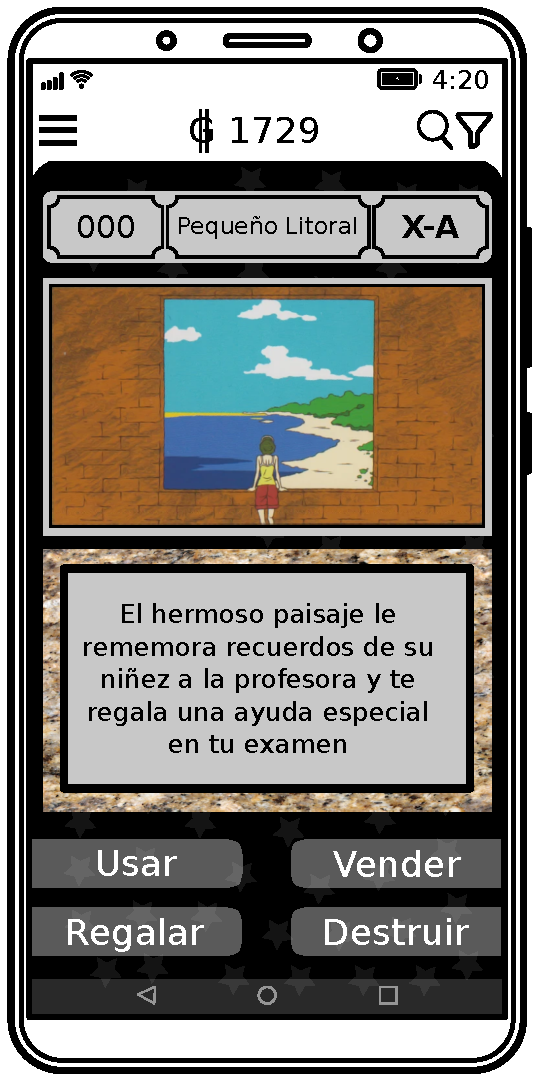
\includegraphics[width=7cm]{prototipos/prototipo1}};
	\draw[red, line width=0.4mm] (-3.05cm, 5cm) rectangle (-2.4cm, 5.65cm) {};
	\draw[red, line width=0.4mm] (-4cm, 5.32cm) -- (-3.05cm, 5.32cm);
	\node[red, anchor=east] at (-4.05cm, 5.32cm) {\textlangle A\textrangle\ Menú de navegación};
	\draw[red, line width=0.4mm] (2.4cm, 5cm) rectangle (2.9cm, 5.65cm) {};
	\draw[red, line width=0.4mm] (2.9cm, 5.32cm) -- (4cm, 5.32cm);
	\node[red, anchor=west] at (4.05cm, 5.32cm) {\textlangle B\textrangle\ Menú de filtro};
	\draw[red, line width=0.4mm] (1.9cm, 5cm) rectangle (2.4cm, 5.65cm) {};
	\draw[red, line width=0.4mm] (2.15cm, 5.65cm) -- (2.15cm, 6.5cm);
	\draw[red, line width=0.4mm] (2.15cm, 6.5cm) -- (4cm, 6.5cm);
	\node[red, anchor=west] at (4.05cm, 6.5cm) {\textlangle C\textrangle\ Menú de búsqueda};
	\draw[red, line width=0.4mm] (-1.4cm, 5cm) rectangle (1cm, 5.65cm) {};
	\draw[red, line width=0.4mm] (-0.2cm, 5.65cm) -- (-0.2cm, 7.5cm);
	\node[red, anchor=south] at (-0.2cm, 7.5cm) {\textlangle D\textrangle\ Indicador divisa virtual};
	\draw[red, line width=0.4mm] (-3.05cm, -3.6cm) rectangle (2.95cm, 4.7cm) {};
	\draw[red, line width=0.4mm] (-4cm, 0.55cm) -- (-3.05cm, 0.55cm);
	\node[red, anchor=east] at (-4.05cm, 0.55cm) {\textlangle E\textrangle\ Zona de las cartas};
	\draw[red, line width=0.4mm] (-3.05cm, -5.5cm) rectangle (2.95cm, -3.7cm) {};
	\draw[red, line width=0.4mm] (-4cm, -4.6cm) -- (-3.05cm, -4.6cm);
	\node[red, anchor=east] at (-4.05cm, -4.6cm) {\textlangle F\textrangle\ Zona de controles};
\end{tikzpicture}
